\section{Complexidade}
\textbf{O que é a complexidade de um algoritmo?}

Complexidade de algoritmo refere-se à medida de eficiência de um algoritmo em termos de tempo e espaço. Ela avalia o quanto de recurso computacional (como CPU ou memória) que um algoritmo requer para resolver o problema conforme sua entrada cresce. A complexidade é geralmente expressa na notação Big O, que descreve o comportamento assintótico do algoritmo ao considerar o tamanho da entrada para um pior caso. Por exemplo, um algoritmo com complexidade O(n) tem um tempo de execução que cresce linearmente com o tamanho da entrada, enquanto um com complexidade $O(n^2)$ tem um tempo de execução com crescimento quadrático.

Existem dois tipos principais de complexidade: complexidade de tempo e complexidade de espaço. A complexidade de tempo se refere à quantidade de tempo que um algoritmo leva para processar uma entrada de tamanho n, enquanto a complexidade de espaço se refere à quantidade de memória necessária. Entender a complexidade ajuda na escolha de algoritmos mais eficientes, especialmente para grandes conjuntos de dados, permitindo soluções que equilibram entre rapidez e uso de recursos, fundamental para otimização em desenvolvimento de software e ciência da computação.

\subsection*{Notação $O$}
    Quando existe um limite assintótico superior, a notacão $O$,é utilizada. Para uma dada função g(n), denotamos por O((g(n)) (lê-se "Ó grande de g de n" ou, "ó de g de n") o conjunto de funções $O(g(n)) =f(n)$( existem constantes positivas $c$ e $n_0$ tais que $0\leq f(n) \leq c*g(n)$ para todo $ n \geq n_0$).
    
Usamos a notação $O$ para dar um limite superior a uma função, dentro de um fator constante. Para todos os valores $n$ em $n_0$ ou à direita de $n_0$, o valor da função $f(n)$ está abaixo de $c*g(n)$.

 Tendo em vista que a notação $O$ descreve um limite superior, quando a empregamos para limitar o tempo de execução do pior caso de um algoritmo temos um limite para o tempo de execução do algoritmo em cada entrada\cite{AlgoritmoCormen2009}.




\subsection{Complexidade O(1)}

A complexidade $O(1)$, ou complexidade de tempo constante, significa que um algoritmo leva o mesmo tempo para executar, independentemente do tamanho da entrada. Isso ocorre porque o algoritmo realiza um número fixo de operações, como calcular a distância entre dois pontos ou acessar um elemento específico em matrizes.

A fim de  demonstrar o sistema de complexidade $O(1)$ será utilizado um exemplo como base, neste exercício  é necessário criar um programa que quantifique diferentes tipos de pisos para uma sala qualquer, onde não basta apenas ter área da sala, pois os pisos se diferem entre inteiros e cortados, então leva-se em consideração os espaços não completos do chão da sala.

A complexidade $O(1)$, trabalha com uma constante durante todo o seu processo, para fins de contagem a constante é desprezada.
Segue o exemplo:
\newpage
\begin{center}
Piso da escola

{ OBI 2018}

Timelimit: $1$	
\end{center}

 O colégio pretende trocar o piso de uma sala de aula e a diretora aproveitou a oportunidade para passar uma tarefa aos alunos. A sala tem o formato de um retângulo de largura $L$ metros e comprimento $C$ metros, onde $L$ e $C$ são números inteiros. A diretora precisa comprar lajotas de cerâmica para cobrir todo o piso da sala. Seria fácil calcular quantas lajotas seriam necessárias se cada lajota fosse um quadrado de $1$ metro de lado. O problema é que a lajota que a diretora quer comprar é um quadrado que possui $1$ metro de diagonal, não de lado. Além disso, ela quer preencher o piso da sala com as diagonais das lajotas alinhadas aos lados da sala, como na figura.

A loja vai fornecer lajotas do tipo $1$: inteiras; do tipo $2$, que correspondem à metade das do tipo $1$, cortadas ao longo da diagonal; e lajotas do tipo $3$, que correspondem à metade do tipo $2$. Veja os três tipos de lajotas na figura.

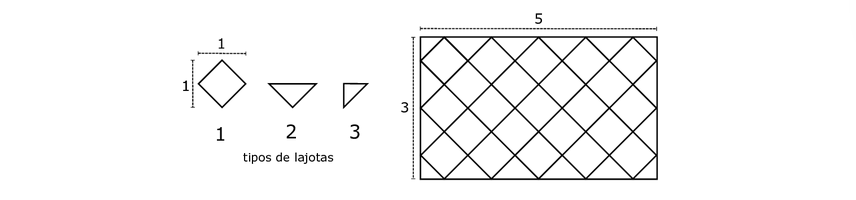
\includegraphics[width=1.0\textwidth]{fig/Piso da Escola.png}
 Está muito claro que sempre serão necessárias $4$ lajotas do tipo $3$ para os cantos da sala. A tarefa que a diretora passou para os alunos é calcular o número de lajotas dos tipos $1$ e $2$ que serão necessárias. Na figura, para $L=3$ e $C=5$, foram necessárias $23$ do tipo $1$ e $12$ do tipo $2$.

Seu programa precisa computar, dados os valores de $L$ e $C$, a quantidade de lajotas do tipo $1$ e do tipo $2$ necessárias.

\vspace{0.3cm}
\textbf{Entrada}

A entrada consiste de um único número inteiro $L$ indicando a largura da sala. A segunda linha contém um inteiro $C$ representando o comprimento da sala, conforme dados da tabela~\ref{tabela01}. 

\vspace{0.3cm}
\textbf{Saída}

Imprima duas linhas na saída. A primeira deve conter um inteiro, representando o número de lajotas do tipo $1$ necessárias. A segunda deve conter um inteiro, indicando o número de lajotas do tipo $2$.

\textbf{Restrições}
\begin{itemize}
    \item $1 \leq L,C \leq 100$
\end{itemize}

\begin{table}[!ht]
    \centering
    \begin{tabular}{|p{7cm}|p{7cm}|}
        \hline
        \begin{center}
            \vspace{-0.3cm}
            \textbf{Exemplos de Entrada}
            \vspace{-0.3cm}
        \end{center} 
         &  
        \begin{center}
            \vspace{-0.3cm}
            \textbf{Exemplos de Saída}
            \vspace{-0.3cm}
        \end{center} \\ \hline
         \texttt{3} & \texttt{23} \\
         \texttt{5} & \texttt{12} \\
         \hline
         \texttt{1} & \texttt{1} \\
         \texttt{1} & \texttt{0}\\
         \hline
    \end{tabular}
    \caption{Exemplos de entradas e saídas}
    \label{tabela01}
\end{table}

%---------------------------------------------


\begin{table}[ht]
\centering

\label{tab:algoritmo1}
\begin{tabular}{|p{8cm}|c|c|}
\hline
\textbf{\cellcolor[HTML]{C0C0C0}Algoritmo} & \textbf{\cellcolor[HTML]{C0C0C0}Custo} & \textbf{\cellcolor[HTML]{C0C0C0}Complexidade} \\
\hline
\begin{minipage}{8cm}
{
        \begin{algorithm}[H]
            \caption{Piso da Sala}
            \label{alg:01}
            \SetAlgoLined
          \small  \Inicio{
            \textit{Declare} $L, C, T1, T2$ \textit{inteiro} \\
                \textit{Leia} $T1, T2$ \\
                $T1 \leftarrow L * C + ( L - 1) * ( C - 1)$ \\
                $T2 \leftarrow ( L - 1) * 2 + ( C - 1) * 2$ \\
                \textit{Escreva} $T1$ \\
                \textit{Escreva} $T2$ \\
                }
        \end{algorithm}}
\end{minipage} 
& 
\begin{minipage}{2cm}

C1 \\
C2\\
C3 \\
C4 \\
C5 \\
C6 \\
C7 \\
C8 \\
K\\
\end{minipage}
&
\begin{minipage}{2cm}

O(1) \\
O(1) \\
O(1) \\
O(1) \\
O(1)\\
O(1)\\
O(1) \\
O(1) \\
O(1)\\

\end{minipage}
\\
\hline
\end{tabular}
\end{table}


\begin{equation}
T(n)=({C_1}*1)+({C_2}*1)+({C_3}*1)+({C_4}*1)+({C_5}*1)+({C_6}*1)+({C_7}*1)+({C_8}*1)
\end{equation}

\begin{equation}T(n)=({C_1}+{C_2}+{C_3}+{C_4}+{C_5}+{C_6}+{C_7}+{C_8})*1\end{equation}
\begin{equation}\textit{Considere K} = {C_1}+{C_2}+{C_3}+{C_4}+{C_5}+{C_6}+{C_7}+{C_8}\end{equation}

\begin{equation}
    T(n)= K*1 = O(1)
\end{equation}
\begin{center}
\begin{minipage}{0.5\textwidth}
    \lstinputlisting[language=C++]{code/piso1.cpp}
\end{minipage}
\end{center}
\newpage

\subsection{Complexidade O(n)}
Uma complexidade $O(n)$ (complexidade linear) significa que o tempo ou espaço necessário para executar um algoritmo aumenta de forma linear com o tamanho da entrada. Em outras palavras, se você dobrar o tamanho da entrada, o algoritmo também dobrará em tempo de execução ou espaço de memória.

Para demonstrar a complexidade $O(n)$ um exercício retirado do site~\cite{beecrowd1} de busca em um vetor foi escolhido, a atividade em questão consiste em procurar dentro de uma lista de números qual é o menor valor entre eles, destacando também a sua posição dentro da lista.

\begin{center}
\large Menor e Posição

{ BeeCrowd 1180}

Timelimit: $1$	
\end{center}

Faça um programa que leia um valor $N$. Este $N$ será o tamanho de um vetor $X[N]$. A seguir, leia cada um dos valores de X, encontre o menor elemento deste vetor e a sua posição dentro do vetor, mostrando esta informação.

\vspace{0.3cm}
\textbf{Entrada}

A primeira linha de entrada contém um único inteiro $N (1 < N < 1000)$, indicando o número de elementos que deverão ser lidos em seguida para o vetor $X[N]$ de inteiros. A segunda linha contém cada um dos $N$ valores, separados por um espaço. Vale lembrar que nenhuma entrada haverá números repetidos.

\vspace{0.3cm}
\textbf{Saída}
A primeira linha apresenta a mensagem “Menor valor:” seguida de um espaço e do menor valor lido na entrada. A segunda linha apresenta a mensagem “Posição:” seguido de um espaço e da posição do vetor na qual se encontra o menor valor lido, lembrando que o vetor inicia na posição zero.

\begin{table}[!ht]
    \centering
    \begin{tabular}{|p{7cm}|p{7cm}|}
        \hline
        \begin{center}
            \vspace{-0.3cm}
            \textbf{Exemplos de Entrada}
            \vspace{-0.3cm}
        \end{center} 
         &  
        \begin{center}
            \vspace{-0.3cm}
            \textbf{Exemplos de Saída}
            \vspace{-0.3cm}
        \end{center} \\ \hline
         \texttt{10} & \texttt{Menor valor: -5} \\
         \hline
         \texttt{1,2,3,4,-5,6,7,8,9,10} & \texttt{Posicao: 4} \\
         \hline
    \end{tabular}
    \caption{Exemplos de entradas e saídas}
    \label{tabela02}
\end{table}



\begin{table}[ht]
\centering
\caption{Exemplos de entradas e saídas}
\label{tab:algoritmo2}
\begin{tabular}{|p{8cm}|c|c|}
\hline
\textbf{\cellcolor[HTML]{C0C0C0}Algoritmo} & \textbf{\cellcolor[HTML]{C0C0C0}Custo} & \textbf{\cellcolor[HTML]{C0C0C0}Complexidade} \\
\hline
\begin{minipage}{8cm}
\begin{algorithm}[H]
 \caption{Menor e Posicao}
\SetAlgoLined
Declare $X, N, M, POS$ inteiro\;
Leia $N$\;
\For{$X \leftarrow 0$ \textbf{até} $N-1$ faça}{
    Leia $P[X]$\;
}
$M \leftarrow 0$\;
\For{$X \leftarrow 1$ \textbf{até} $N-1$ faça}{
    \If{$P[X] < P[M]$}{
        $M \leftarrow X$\;
    }
}
Escreva $P[M]$\;
Escreva $M$\;
\end{algorithm}
\end{minipage} 
& 
\begin{minipage}{2cm}
C1 \\
C2\\
C3 \\
C4 \\
C5 \\
C6 \\
C7 \\
C8 \\
C9 \\
    C10 \\
C11 \\
C12 \\
C13
\end{minipage}
&
\begin{minipage}{2cm}
1 \\
1 \\
1 \\
1 \\
$n$ \\
$n$ \\
1 \\
$n-1$ \\
$n-1$ \\
$n-1$ \\
$n-1$ \\
1 \\
1
\end{minipage}
\\
\hline
\end{tabular}
\end{table}


\begin{equation}
T(n) = C_1*1 + C_2*1 + C_3*1 + C_4*(n+1) + C_5*n + C_6*1+ C_7*1 + C_8*n
\end{equation}
\begin{equation}
+ C_9*(n-1) + C_10*(n-1) + C_11*1 + C_12*1 + C_13*1 +  C_14*1 + C_15*1
\end{equation}
\begin{equation}
    T(n)= K*(1 + 1 + 1 + n+1 + n + n + 1 + n + n-1 + n-1 + n-1 + n-1 + 1 + 1 + 1)
    \end{equation}
    \begin{equation}
    T(n)= 8*n + 4 =O(n)
    \end{equation}
\begin{center}
\begin{minipage}{0.5\textwidth}
    \lstinputlisting[language=C++]{code/resol++.cpp}
\end{minipage}
\end{center}


    
    \newpage



\subsection{Complexidade O(n²)}

A complexidade O(n²) é uma medida de desempenho de algoritmos que indica que o tempo de execução cresce quadraticamente com o tamanho da entrada, representado por $'n'$. Isso significa que, se o tamanho da entrada dobrar, o tempo de execução será aproximadamente quatro vezes maior, devido ao fator quadrático. Algoritmos com essa complexidade frequentemente envolvem dois loops aninhados, onde cada elemento da entrada é comparado ou processado em relação a todos os outros elementos.

Um exemplo clássico de algoritmo com complexidade O(n²) é o Bubble Sort, onde, para cada elemento de uma lista, são feitas comparações com os elementos subsequentes para realizar trocas e ordenar os dados. Em um caso médio ou pior, o algoritmo precisa percorrer a lista n vezes, e em cada iteração, realiza até n comparações ou operações, resultando em n * n = n² aoperações. Essa característica torna esses algoritmos ineficientes para grandes volumes de dados, pois o custo computacional aumenta rapidamente.

Embora algoritmos O(n²) sejam menos eficientes do que aqueles com complexidades lineares O(n) ou logarítmicas O(log n), eles ainda têm utilidade em cenários com entradas pequenas ou quando a simplicidade de implementação é mais importante que o desempenho. Além disso, podem servir como base para otimizações ou em situações específicas onde o pior caso raramente ocorre. No entanto, para aplicações de larga escala, é comum buscar alternativas mais eficientes, como algoritmos com complexidade O(n log n), típicos de métodos de ordenação mais avançados como Quick Sort ou Merge Sort.

Segue o exemplo representativo da complexidade O(n²):
\begin{center}
Fibonacci em Vetor

{Beecrowd 1176}

Timelimit: $1$	
\end{center}

Faça um programa que leia um valor e apresente o número de Fibonacci correspondente a este valor lido. Lembre que os 2 primeiros elementos da série de Fibonacci são 0 e 1 e cada próximo termo é a soma dos 2 anteriores a ele. Todos os valores de Fibonacci calculados neste problema devem caber em um inteiro de 64 bits sem sinal.

\vspace{0.3cm}
\textbf{Entrada}

A primeira linha da entrada contém um inteiro T, indicando o número de casos de teste. Cada caso de teste contém um único inteiro N $(0 \leq N \leq 60)$, correspondente ao N-esimo termo da série de Fibonacci.

\vspace{0.3cm}
\textbf{Saída}

Para cada caso de teste da entrada, imprima a mensagem "Fib(N) = X", onde X é o N-ésimo termo da série de Fibonacci.

%---------------------------------------------------------

\begin{table}[!ht]
    \centering
    \begin{tabular}{|p{7cm}|p{7cm}|}
        \hline
        \begin{center}
            \vspace{-0.3cm}
            \textbf{Exemplos de Entrada}
            \vspace{-0.3cm}
        \end{center} 
         &  
        \begin{center}
            \vspace{-0.3cm}
            \textbf{Exemplos de Saída}
            \vspace{-0.3cm}
        \end{center} \\ \hline
         \texttt{3} & \texttt{FIB(0) = 0} \\
         \texttt{0} & \texttt{FIB(4) = 3} \\
         \texttt{4} & \texttt{FIB(2) = 1} \\
         \texttt{2} & \texttt{}\\
         \hline
    \end{tabular}
    \caption{Exemplos de entradas e saídas}
    \label{tabela04}
\end{table}
%------------------------------------


\begin{center}
\begin{minipage}{0.5\textwidth}
    \lstinputlisting[language=C++]{fig/fibo.cpp}
\end{minipage}
\end{center}
$T(n)=C1*1+C2*1+C3*1+C4*(59)+C5*T+C6*T$\\
$T(n)=K+(C5+C6)*T$\\
$T(n)=a*T+b=O(T)$

\input{FundamentoAnálise/EA}
\input{FundamentoAnálise/ED}